\chapter{Statistical Simulation for Spatial Sampling}

The angle increment was derived in section \ref{sec:spasa} and is presented in equation \ref{eq:angle}. To find a compromise between measurement speed and accuracy a compromise has to be found for the error generated by spatial aliasing. 

\section{Implementation}

The simulation is similar to section \ref{sec:spasa} done with the \ac{AF}, however with a two dimensional rectangular $\sfrac{\lambda}{2}$-element spacing array. This brings the advantage that the array size can easily be adjusted. The \ac{FF}-pattern is computed with the Matlab\texttrademark{} class \textit{phased.URA}. Here also a steering vector, consistent of an azimuth and an elevation angle, to specify which direction the main beam of the array is facing. The sampling of the \ac{FF}-pattern is accomplished by the included \textit{pattern(...)} function.\\
This simulation is mainly developed for \acp{CSSG} and the angle increment is computed by equation \ref{eq:angle}. With the number of elements in $z$ direction $N_z$ and the number of elements in $y$ direction $N_y$ the radii $r_s$ and $r_c$ can be computed as

\begin{equation}
2r_s = \sqrt{\left(N_y-1\right)^2+\left(N_z-1\right)^2}\cdot\frac{\lambda}{2},\quad 2r_c=\left(N_y-1\right)\cdot\frac{\lambda}{2},
\end{equation}

resulting in an angle increment of

\begin{equation}
\Delta\Theta^\prime = \frac{\text{SF}\cdot\text{CrefA}\left(\sfrac{2r_s}{\lambda}\right)\cdot 2}{\sqrt{\left(N_y-1\right)^2+\left(N_z-1\right)^2}}\ ,\quad\Delta\Phi^\prime = \frac{\text{SF}\cdot\text{CrefA}\left(\sfrac{2r_c}{\lambda}\right)\cdot 2}{\left(N_y-1\right)}.
\end{equation}

Whereby \ac{CrefA} is a function of diameter in wavelength, compare figure \ref{fig:crefa}. The number of points on each longitude half circle $N_\Theta$ and on each latitude circle $N_\Phi$ is computed and round up:

\begin{equation}
N_\Theta = \bigg\lceil\frac{\pi}{\Delta\Theta^\prime}\bigg\rceil ; \quad N_\Phi^\prime = \bigg\lceil\frac{2\pi}{\Delta\Phi^\prime}\bigg\rceil
\end{equation}

For more sparse sampling at the poles the \ac{CTF} with a value range of $\text{CTF}=\left[0,1\right]$ is introduced to gain Theta dependent azimuth step size:

\begin{equation}
N_\Phi\left(\Theta\right) = \bigg\lceil\frac{2\pi}{\Delta\Phi^\prime}\left(1-\text{CTF}+\text{CTF}\cdot\cos\right(\Theta\left)\right)\bigg\rceil
\end{equation}

For easier computation $N_\Phi\left(\Theta\right)$ is round to 

\begin{equation}
N_\text{round} = \bigg\lceil \frac{N_\Phi^\prime}{k} \bigg\rceil, \ k \in \mathbb{N}
\end{equation}

and not just to the greater integer. So that the angle increment is

\begin{equation}
\Delta\Theta = \frac{\pi}{N_\Theta} , \quad \Delta\Phi\left(\Theta\right) = \frac{2\pi}{N_\Phi\left(\Theta\right)}.
\end{equation}

With the integers in $N_\text{round}$ the advantage is that a uniform \ac{CSSG} can be sampled and the theta dependent phi can be simulated by discarding every $k$th value in each azimuth circle.

\section{Set Up}

\begin{figure}
  \centering
  \subfigure[PDF]{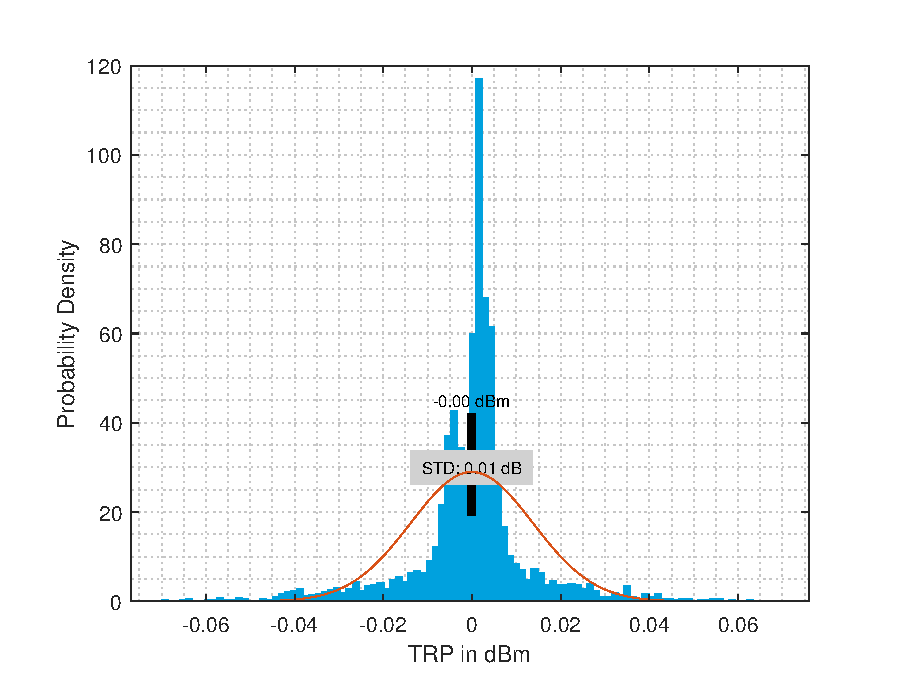
\includegraphics[width=0.49\textwidth]{Matlab/PDF_6-18_SF1.eps}}
  \centering
  \subfigure[CDF]{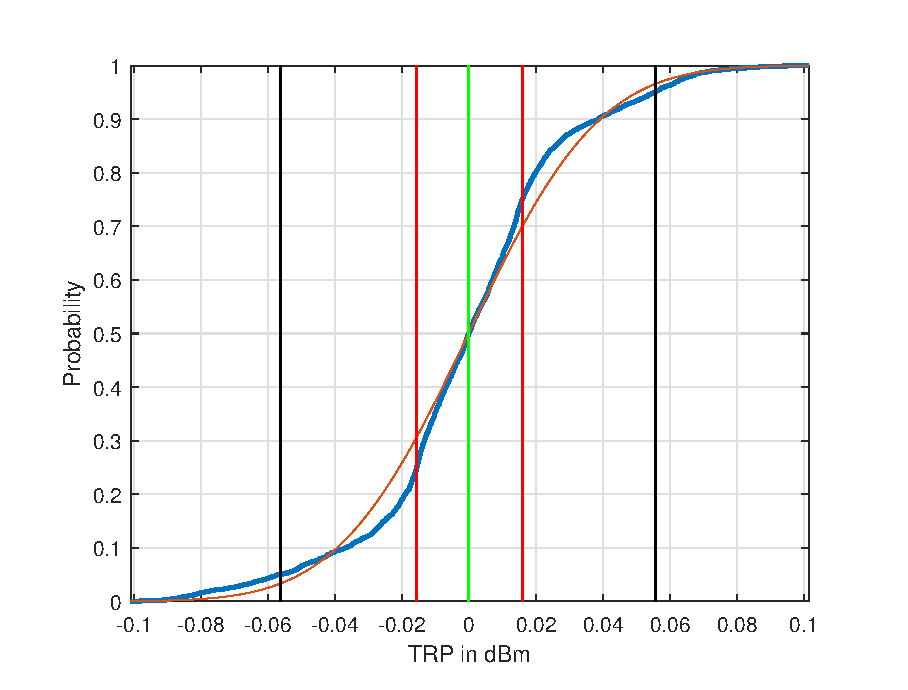
\includegraphics[width=0.49\textwidth]{{Matlab/CDF_6-18_SF1.eps}}}
\caption{4000 random steering vectors, $\text{SF}=1$, 6x18-Array}
\label{fig:rands}
\end{figure}

Summarising there are four input parameters first the \ac{SF}, second the \ac{CTF} and third and fourth the elements of the array in $y$ and $z$ direction. Every set of parameters is simulated with $N=4000$ samples. The azimuth steering is evenly distributed over the whole circle from $-\pi$ to $\pi$. In elevation a random variable is generated with a \ac{CDF} of \ac{CC} coefficients from $-\sfrac{\pi}{2}$ to $\sfrac{\pi}{2}$ by projecting evenly distributed random numbers. With that the main beam direction is evenly distributed over the spheres surface. For every set of parameters the following third step iterated $N$ times:

\begin{enumerate}
\item Generate $N$ steering vectors.
\item Derive a \ac{CSSG}.
\item Compute the \ac{TRP}:
\begin{enumerate}
\item Generate a antenna pattern using a random steering vector. A sample for that is depicted in figure \ref{fig:randp}.
\item Sample the antenna pattern with the derived grid.
\item Discard samples dependent on the \ac{CTF}.
\item Compute a \ac{TRP} using the \ac{CC}-quadrature.
\end{enumerate}
\end{enumerate}

A histogram and the resulting cumulative frequency diagram is plotted in figure \ref{fig:rands} (a) and (b). In both diagrams additionally the \ac{PDF}, respectively \ac{CDF} of the normal distribution is plotted in orange. Because the normal distribution is not a accurate metric for the underlying distribution, the $\SI{90}{\percent}$ \ac{IQR}, from the $\SI{5}{\percent}$ quantile to the $\SI{95}{\percent}$ quantile, is used to describe the scattering. In figure \ref{fig:rands} (b) the black lines are the $\SI{5}{\percent}$- and $\SI{95}{\percent}$- quantiles, the red lines the $\SI{25}{\percent}$- and $\SI{75}{\percent}$- quantiles and the mean is the green line.\\
The 

\section{Result}